\documentclass[10pt]{article}
\usepackage[margin=0.8in]{geometry}
\usepackage{graphicx}
\usepackage[T1]{fontenc}
\usepackage[hidelinks]{hyperref}
\setlength{\parindent}{0pt}
\setlength{\parskip}{6pt}
\begin{document}
{\LARGE Backend and algorithm frontier}\par
{\large Initial integration and validation --- 17 October 2026}

\textbf{Delivered.} A standalone native Rust report imports 17 historical
sessions into 626 exact-target backend entries, retaining 170 planned cells
without measurements. F4 matrix, inherited F4, F5 matrix, F6-IC, custom root
finding, SAT and reference methods share one view. No solver was run or retimed.

\textbf{The incumbent to improve.} The IC recipe frontier identifies
nondominated IC configurations on the same exact target, session, rounds and
seeds at all three sensitivity weights (0, 0.1 and 1 GAE per native operation).
The cross-method frontier and memory tradeoffs remain separate. Raw solver
counters retain their units; SAT conflict and learned-clause observations keep
their original JSON source pointer. A stage gain is not a full-operation gain.

\begin{center}
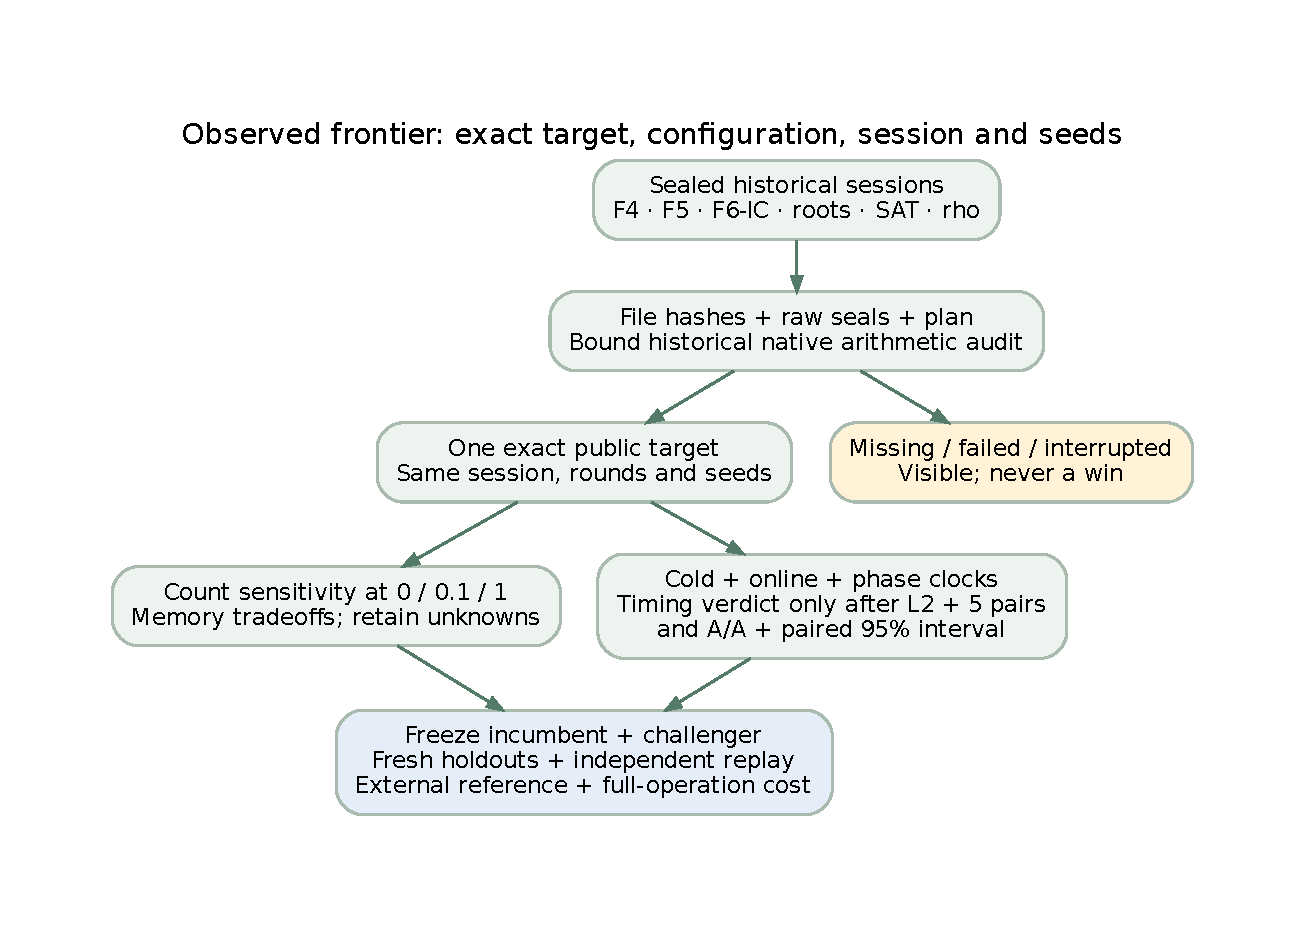
\includegraphics[width=\linewidth,height=8.1cm,keepaspectratio]{flow.pdf}
\end{center}

\textbf{Coverage is evidence, not a study name.} Fields of size
$2^3$, $2^4$, $2^5$, $2^{51}$ and $2^{83}$ have no imported measurements.
Degree 53 does have observations, with their audit limits visible. The study
named \texttt{ecbench\_m83\_rho\_20261005} supplies calibration at degrees
53, 59 and 61; it does not establish degree-83 coverage. Interrupted degree-31
plans stay incomplete. The exact $E_0$ degree-83 scaling gate remains open.

\textbf{Timing and validation.} No timing winner is admitted by this panel's
complete L2, five-pair, same-target A/A and paired-interval gates. The table
shows descriptive cold solve, online, process and phase clocks. Native tests,
lint, read-only freshness checks and desktop/mobile browser checks accompany
the implementation. Historical arithmetic audits must bind the exact source
files; this report performs no fresh arithmetic replay.

\textbf{Existing validation gates.} The root library on base
\texttt{c6d64436} fails compilation (25 ecbench build errors; 26 library-test
compile errors), in unchanged integration files. The existing site suite also
has progress-JSON/panel-index failures and a shallow-input read limitation.
These are recorded in the Markdown report and validation logs, not waived.
The new report builds independently. No global-fastest, external-tool,
asymptotic or ledger-promotion claim is made.

\textbf{Reproduction.} The pinned Rust 1.99.1 producer checks a reviewed
input/output lock (R0). Per-session command cards and the fresh-ledger checker
(R1) require full native audits and exact solver counters, including conflicts
and learned clauses. These checks do not establish an independent execution
or timing equivalence (R2). Fresh runs remain blocked by the root build and
historical source gaps. Exact acceptance criteria:
\texttt{BACKEND\_REPRODUCTION.md}. Commands, evidence and limits:
\texttt{REPORT.md} and \texttt{validation/}. Diagram source: \texttt{flow.dot}.
\end{document}
